
In this section, we present the results of evaluation of our system. As experimental 
setup, we use RTLSDR together with a signal processing algorithm implemented
in Octave. 

\subsection{Spatial variation of ambient television signals}

\begin{figure}[h]
	\centering
	\begin{minipage}{0.49\columnwidth}
	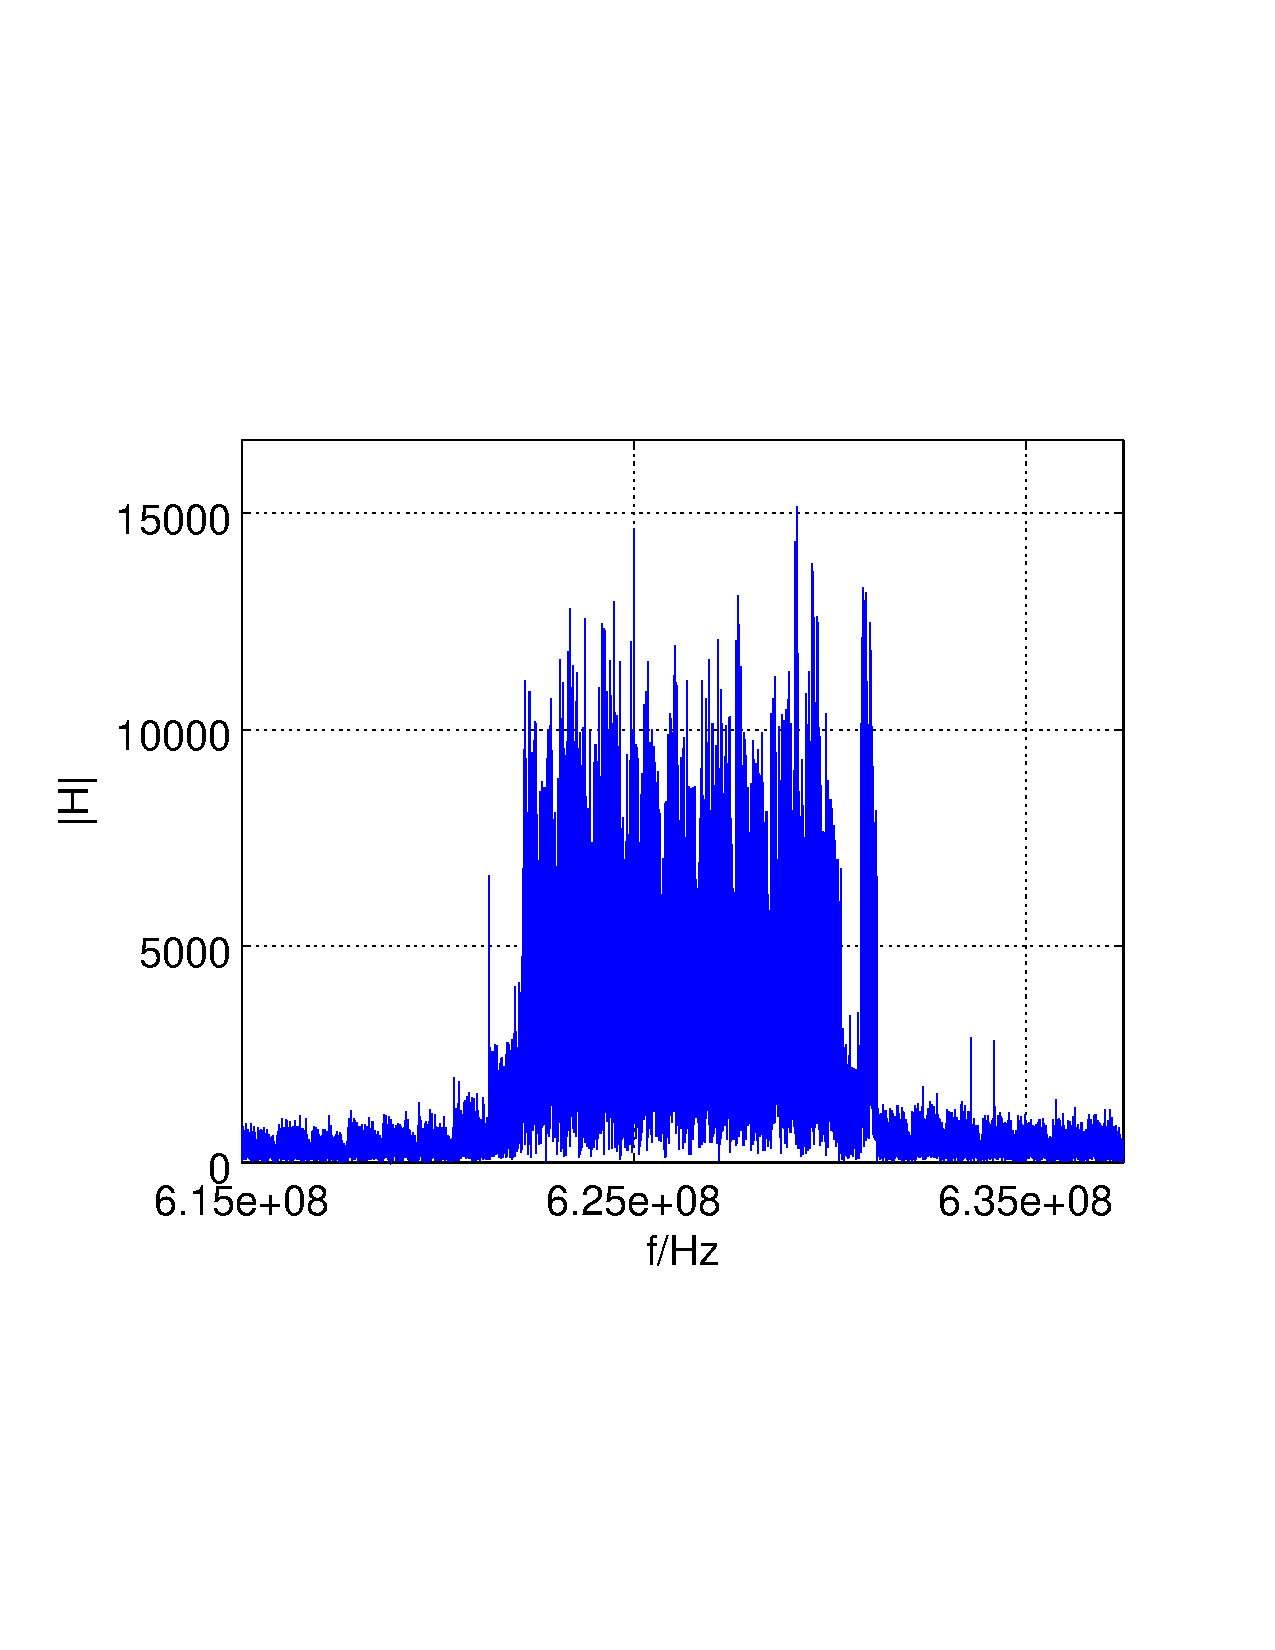
\includegraphics[width=\columnwidth]{./fig/626mhz_raw}
	\end{minipage}
	\hfill
	\begin{minipage}{0.49\columnwidth}
	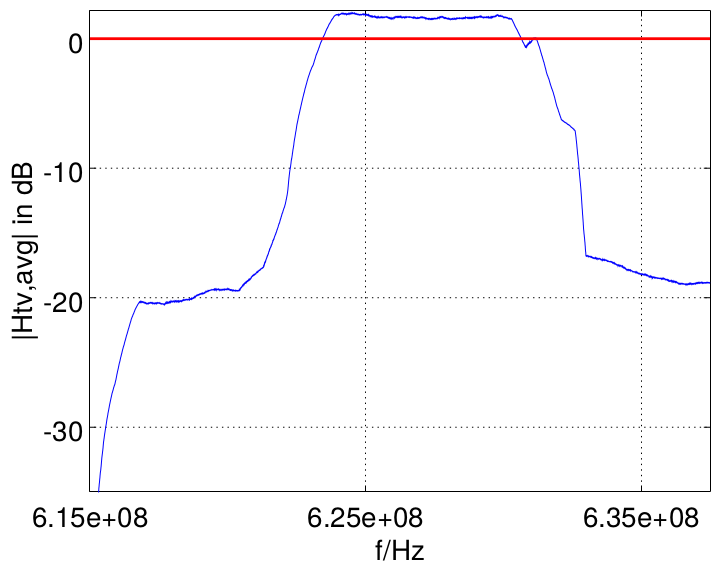
\includegraphics[width=\columnwidth]{./fig/626mhz_filtered}
	\end{minipage}
	\vspace{-6mm}
	\caption{\emph{Observed spectrum of television signal}. The left hand image shows the raw spectrum of the TV signal, with centre frequency of \SI{626}{\mega\hertz}. The right hand image shows the smoothed spectrum normalized to maximum average. The average is  shown by the horizontal red line.}
	\label{fig:tv_record} 
		\vspace{-6mm}
\end{figure}

In this experiment, we investigate the variation of the television signal
in space, i.e., how does the strength of the signal varies over 
the area of the city. We use the RTLSDR reader to obsevre the signal strength.
We perform the frequency sweep of the desired television band. Next, we
obtain the sample in the time domain, and convert them to corresponding
samples in frequency domain by performing fast-fourier transformation~(FFT).

As we are not interested in realtime visualisation of the television
signals, we acquire the signals offline and visualise the samples.
RTLSDR dongle has a maximum sampling rate of 2.4 MS/s, which limits us to
scanning a band of \SI{1.2}{\mega\hertz} band in a single run. We  keep some safety-margin, and
sample the desired band at \SI{900}{\kilo\hertz} intervals. We sample the band 
\SI{20}{\mega\hertz} wide, by stitching individual bands. In our experiments, it takes roughly 30
seconds for us to perform the scanning operation.


%These scripts are available under \cite{s3xm3x_RTLSDRSpecAn}
 
During the scanning process the gain is set to 40.2 dB. To get the
signal strength we simply take the average over a 10 MHz band around the
center frequency of the desired TV signal. This approach can be
justified by the fact, that DVB-T 2 is specified up to 10 MHz bandwidth.
And the local TV provider advertises to be transmitting DVB-T 2.
The signal \ensuremath{|H|} is calculated as follows.  
\begin{equation}
	|H| = \Biggl| \sum_{n=0}^N FFT\biggl( \Re\{ s_{\text{band,n}}(t) \} \biggr) \Biggr|
\end{equation}     where \ensuremath{N} is the total number of intervals
accumulated over the entire frequency sweep. The FFT is only carried out over
the real values, which are received from the \textit{RTL-SDR}.
\ensuremath{s_{\text{band,n}}(t)} is the signal in the time domain of one
interval (one subband). There are as many samples taken in one band as needed
for an FFT of size 2048. To finally get \ensuremath{|H_{tv,avg}|} one has to
normalize everything and calculate the power. Before doing that, a simple
smoothing algorithm (FIR) is applied on \ensuremath{|H|}.  
\begin{equation}
	|H_{\text{tv,avg}}| = 20 \cdot log (|H|) - 20 \cdot log(|H_0|)
\end{equation}   
where \ensuremath{|H_0|} is a normalization value measured at a certain point
in space. 

Figure~\ref{fig:haversine} demonstrates the result of combing the measured
signal strength values, together with the harvesine function enables us to
calculate the distance from the point where maximum signal has been
capture. 

\begin{figure}[h]
	\centering
	\begin{minipage}{0.49\columnwidth}
	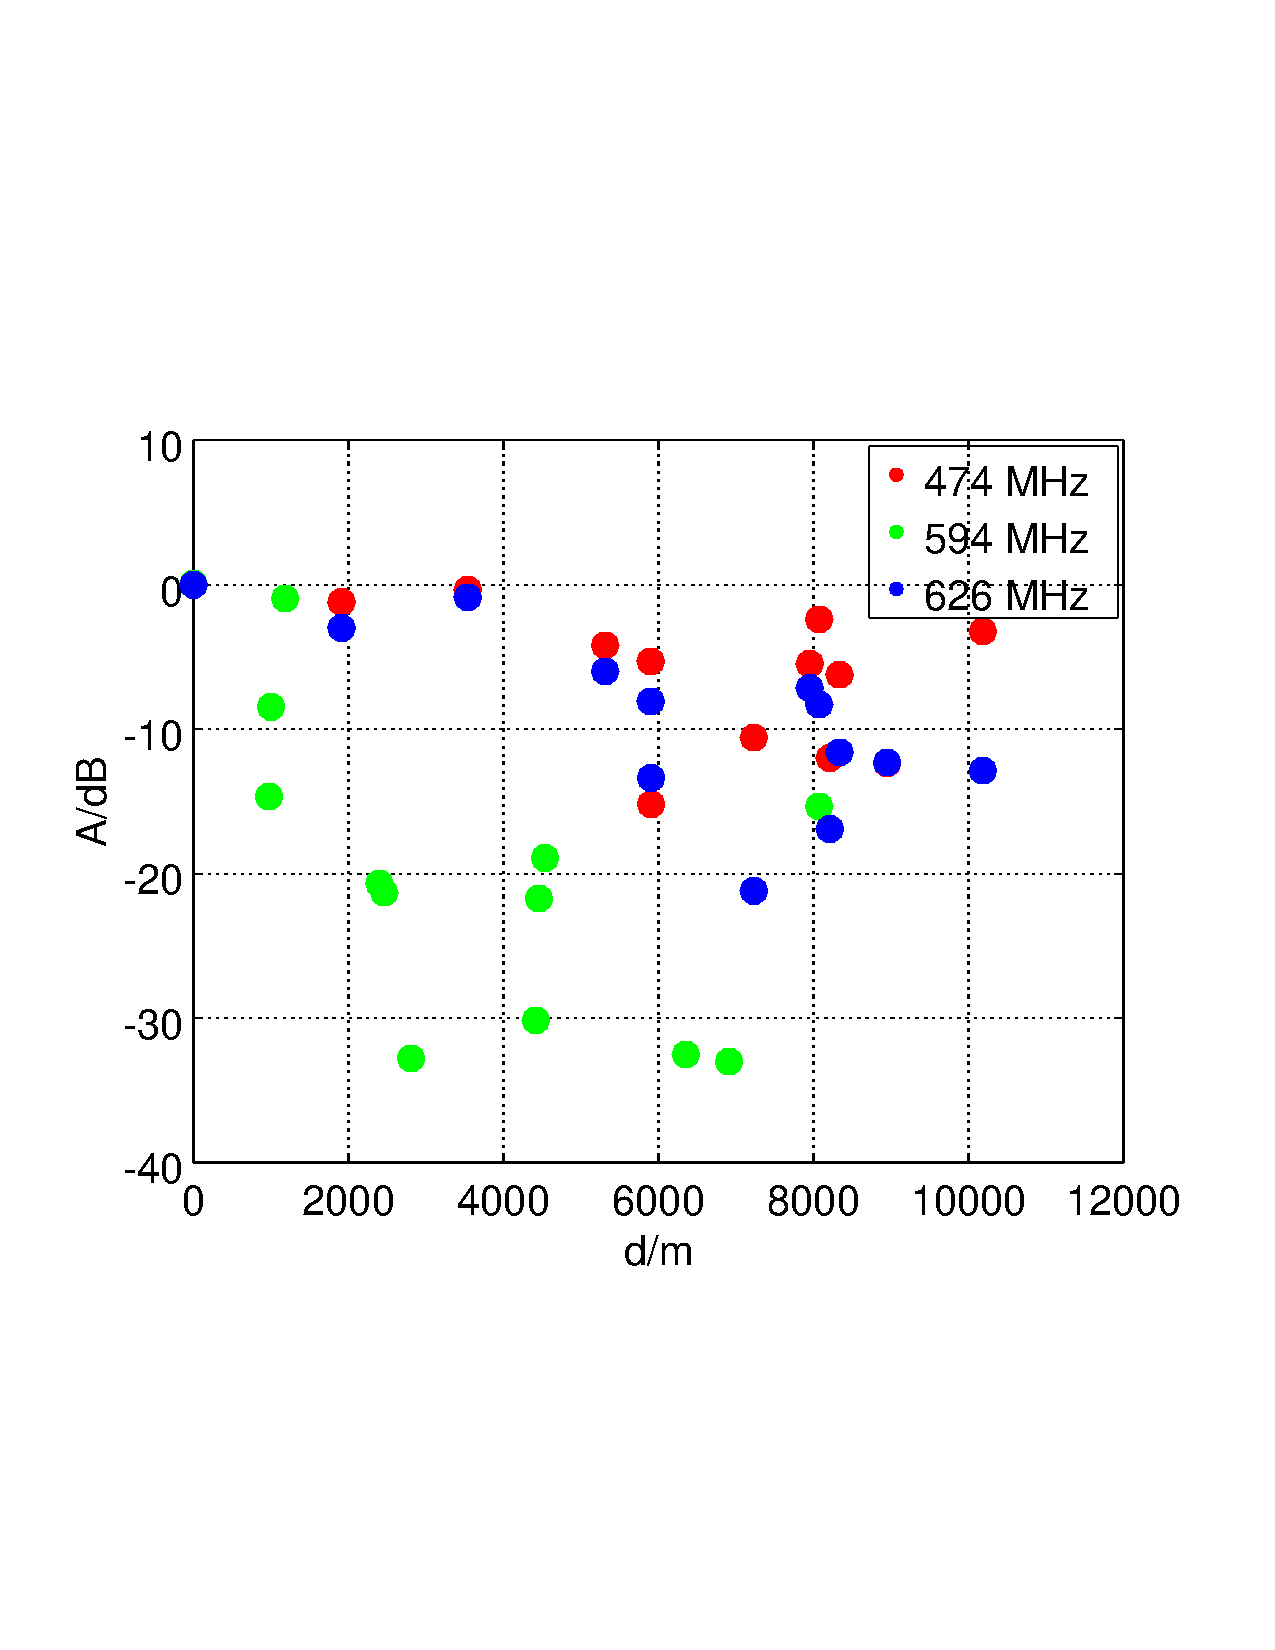
\includegraphics[width=\columnwidth]{./fig/haversine}
	\end{minipage}
	\hfill
	\begin{minipage}{0.49\columnwidth}
	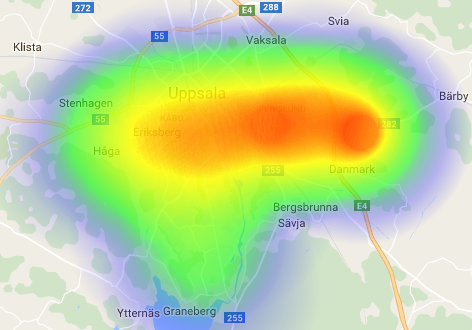
\includegraphics[width=\columnwidth]{./fig/heatmap_626mhz}
	\end{minipage}
	\vspace{-6mm}
	\caption{\emph{Spatial variation of TV signals in Uppsala city}. 
	The left image demonstrates the signal strength of TV signal fading	
	as opposed to observed signal strength near the TV tower. 
	The right image visualises the signal strength as heatmap for the signal
	present in the \SI{626}{\mega\hertz} band. Distances have been
calculated with the Haversine formula. }
 	\vspace{-6mm}

\label{fig:haversine}
\end{figure}

\balance

\subsection{Communication Performance}
In this experiment, we present some preliminary results to evaluate the communication
performance of our system.  In the experiment, we varied the bitrate of the transmitter
from 1 bit/s up to 1 kbit/s. As we had seen earlier in the Figure~\ref{fig:transmission}, the strength
of the backscattered signal is rather low leading to the appearance of significant quantisation noise.
We improve the situation by increasing the analog gain of the receiver, and perform
the experiment with the maximum gain \SI{50}{\decibel} available at out receiver.

In an indoor environment, where the ambient signal strength is low, we are
able to achieve a data rate of 1 b/s with distances of
couple of meters. At higher bitrates, we observe a range of few 
few decimeters and the  bit error rate is still approximately 40 \%. 
We observed similar results outdoors. We acknowledge the high bit errors
observed due to primarily limited gain available on the low cost dongles.
In future, we will work to improve this. We note, existing ambient backscatter
systems do not operate well indoors at large distances, and our results
provide preliminary results of  improvements possible by leveraging low-cost
SDRs.
